% !TeX root = ../Skript_HTML.tex
\cohead{\Large\textbf{Sonderzeichen}}
\section{Umlaute und Sonderzeichen}
Je nach Betriebssystem und Browser kann es zu Problemen bei der Darstellung von Zeichen kommen, insbesondere bei Umlauten:

\begin{minipage}[t]{0.8\textwidth}
    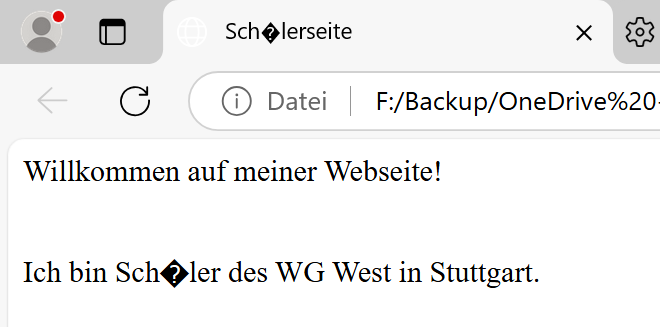
\includegraphics[width=\linewidth]{\pics/Umlaute.png}
\end{minipage}

Um solche Probleme zu vermeiden, ist es empfehlenswert, die Umlaute durch bestimmte Zeichenfolgen, sogenannte Escape-Sequenzen, zu ersetzen, z.B. statt ä im Quellcode \lstinline|\&auml;| zu schreiben. Im Internet lassen sich verschiedenen Listen mit diesen Zeichenfolgen finden.

\begin{Exercise}[title=, label=Umlaute]
    \begin{enumerate}
        \item Füge zwischen den head-Tags (\lstinline|<head> ... </head>|) den folgenden Tag ein: \lstinline|<meta charset="utf-8">|
        \item Schaue dir dann deine Seite nochmals im Browser an.
        \item Ersetze alle Umlaute durch Escape-Sequenzen und verwende in Zukunft diese statt den Umlauten oder dem scharfen s.
        \item Prüfe nochmals im Browser, ob die Umlaute nun alle korrekt dargestellt werden.
        \item Ändere nun noch die Codierung deiner Datei auf UTF-8. Gehe dazu im Editor nochmals auf Speichern unter\(\rightarrow\)Dateityp auf alle Dateien ändern und Codierung auf UTF-8. (Hinweis: Oft wird die Datei standardmäßig bereits mit UTF-8 gespeichert.)
    \end{enumerate}
    \begin{minipage}[t]{\textwidth}
        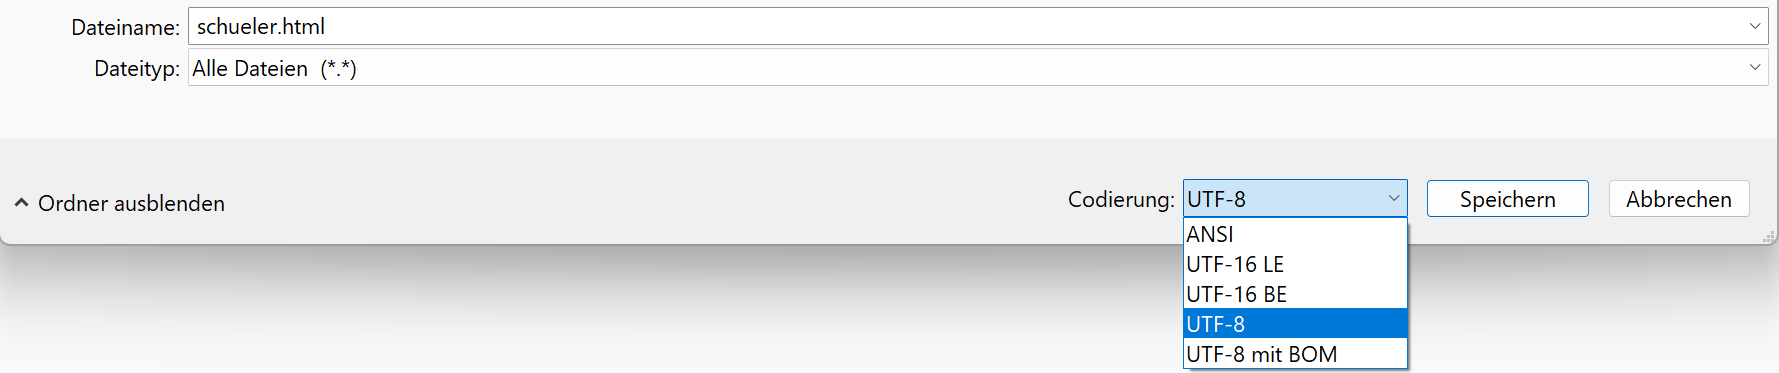
\includegraphics[width=\linewidth]{\pics/UTF8Speichern.png}
    \end{minipage}%
\end{Exercise}